\section{Introduction}

Notation poses a barrier to understanding mathematical ideas. Whether in the physics classroom, data science research papers~\cite{ref:mysore2023how}, or programming documentation~\cite{ref:cai2019software}, readers find important knowledge locked behind the formalisms of formulas and symbols. 
Consider a reader encountering this formula in a research paper \cite{ref:hohman2019gamut}:

% To develop this understanding, learners need to engage with mathematical ideas in the languages that they are expressed. However, when the background of the reader does not match the expectations of the learning material, this could impose a barrier to effective comprehension.

\begin{center}
\vspace{1ex}

\includegraphics[width=0.62\linewidth]{figures/pre-aug-intro}
\end{center}
\vspace{-0.5ex}

This formula represents a linear regression model. If the reader is not familiar with its idioms, they are likely to find it hard to understand. For instance, what is ``$x$'' and how is it different from ``$\beta$''? $\beta_0$ and $\beta_1$ share a common base---how are they related? What is the intuition of the formula as a whole?

Suppose the formula was instead shown as follows:

% \vspace{-.2ex}
\begin{center}
\vspace{0.5ex}
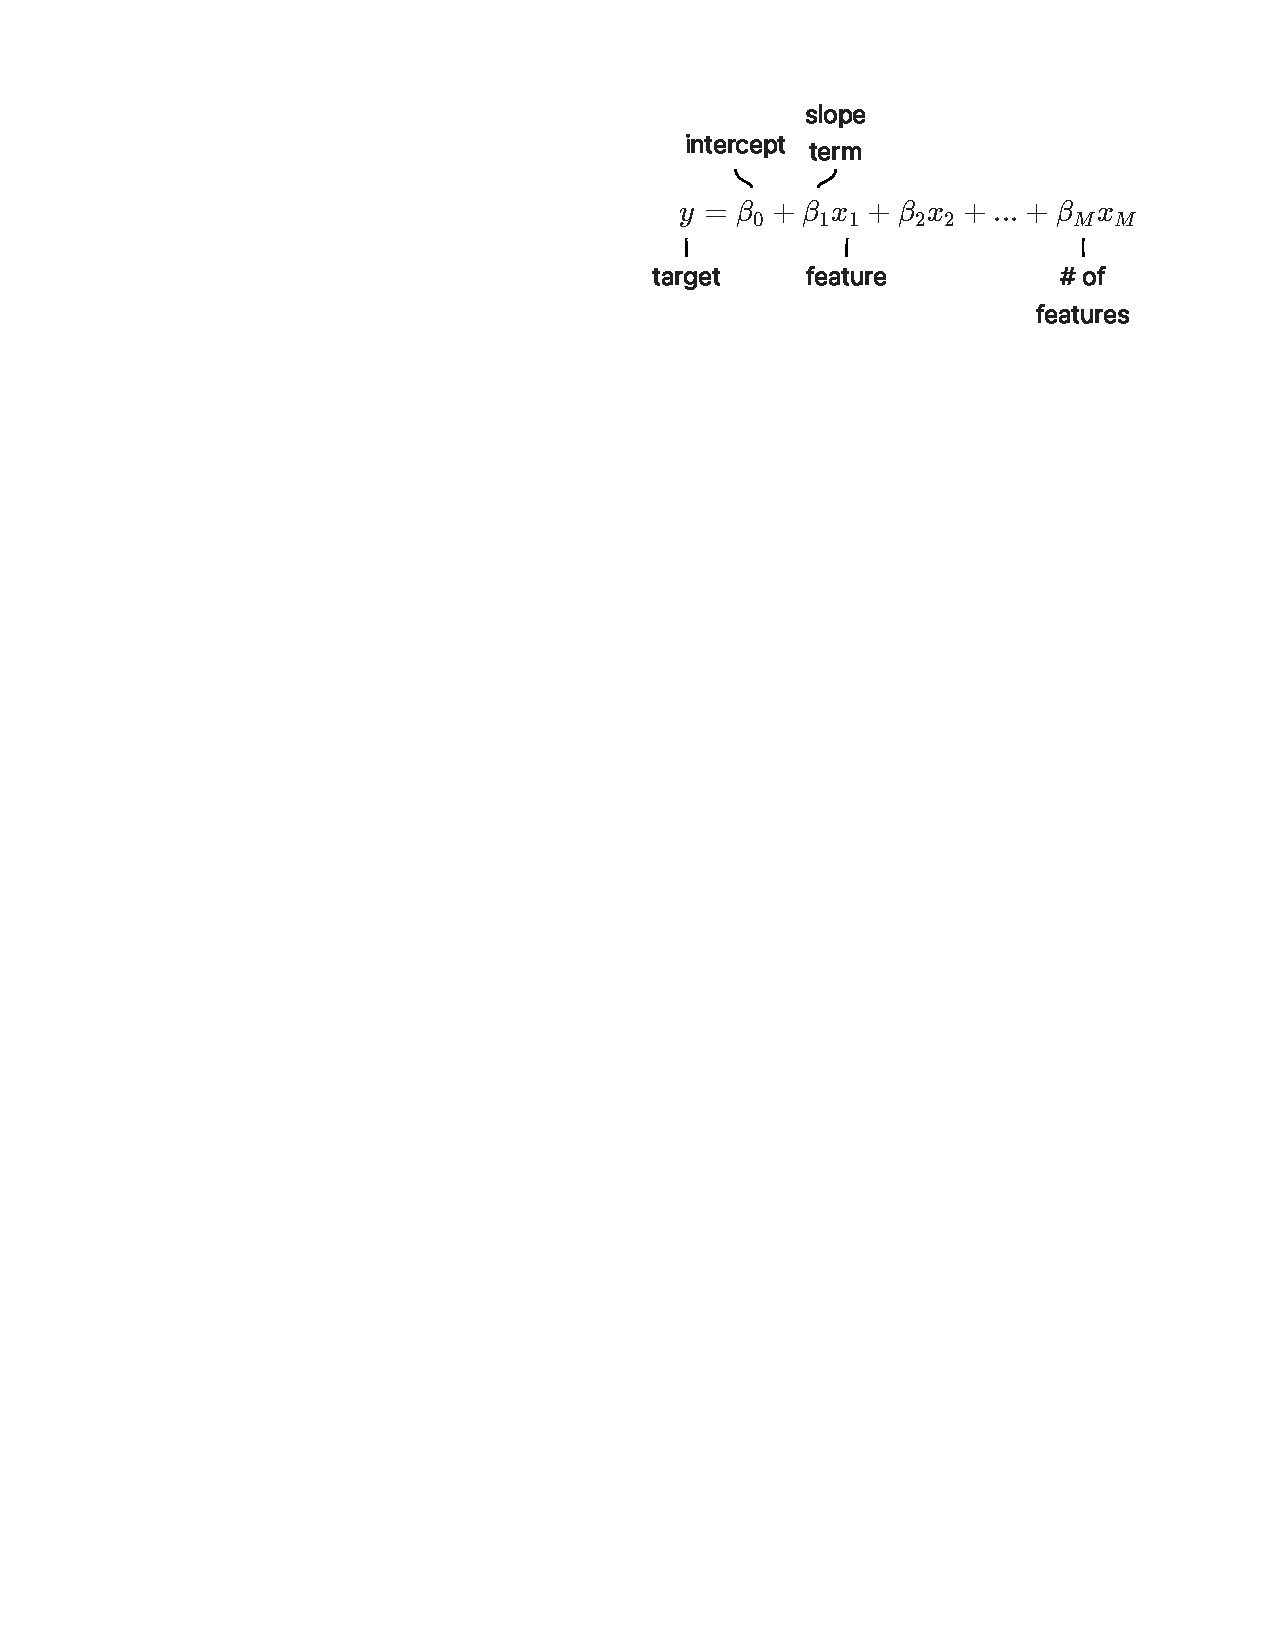
\includegraphics[width=0.65\linewidth]{figures/aug-intro}
\Description{A linear regression formula, augmented with descriptive labels. “y” is labeled “target”; “beta-sub-0” is labeled “intercept”; “beta-sub-1” is labeled “slope term”; “x-sub-1” is labeled “feature”; “beta-sub-M” is labeled “number of features.”}
\vspace{0.5ex}
\end{center}
% \vspace{-.5ex}

This alternative presentation helps a reader to unpack the meaning of a formula. It helps the reader understand the purpose of the formula as predicting a target value from a set of input features. It clarifies that ``$x$'' terms correspond to features, and ``$\beta$'' terms correspond to weights. And it brings the formula into a realm of familiarity by relating ``$\beta_0$'' and ``$\beta_1$'' to the ideas of intercept and slope terms that are taught in algebra class.
Annotated formulas like these help readers grasp their meaning at glance. The annotations' value becomes particularly pronounced when applied to formulas of yet greater complexity and domain specificity.

In this paper, we seek to advance the state of the art in tooling that allows authors to create augmented formulas like these. A recent survey by \citet{ref:head2022math} reveals the challenges present in building effective interactive tooling for this purpose. Conventional formula typesetting tools often make it a ``struggle'' to augment formulas. Formula markup gets too messy, and environments provide insufficient support for experimenting with cross-document formula styling choices.

Our contribution is a reinvention of the process of augmenting formulas in typesetting tools. We envision formula augmentation as a process that involves a crisp markup language and live incremental feedback. We reify this vision in \emph{FFL}, or ``Formula Formatting Language,'' a markup language for formula augmentation. FFL is targeted for web-based math document authoring. Its key innovations are a design that splits augmentation markup from formula markup, a CSS-inspired familiar syntax, support for cross-document styling, and an implementation that permits live feedback.

% In this paper, we envision an improved authoring experience where users are enabled to separate their augmentation and formula specifications, apply augmentations to multiple expressions simultaneously, and rapidly experiment with alternative augmentations. The result is a language called \emph{FFL}, or ``Formula Formatting Language,'' and an accompanying live runtime.

% Here, a reader can easily gauge what each variable stands for, track which terms in the equation are related, and understand their usage in the equation.

% While augmentations facilitate better comprehension, the tools that authors use to present formulas often introduce friction in doing so. In a recent survey, \citet{ref:head2022math} describe that authors find themselves using tools that involve clunky markup languages, ugly defaults, and tedious graphic editing.

% One class of tools that poses friction is markup languages for typesetting formulas. Today, TeX~\cite{ref:knuth1986tex} is perhaps the most widely-used markup language for expressing formulas. Yet, augmenting formulas with a TeX tool requires injecting augmentation code (e.g., color and label macros) into the underlying formula. This results in an experience described a ``struggle''~\cite{ref:head2022math} as markup becomes difficult to read and efficiently edit. Furthermore, unless an author has been disciplined about defining expressions using macros, it can be time-consuming to alter style choices across formulas.

We assess FFL's impact on the authoring experience in a controlled usability study where 28 participants used FFL and \zed{a} LaTeX baseline.
\zed{In complex editing tasks, FFL increased efficiency and self-reported ease, and led to more readable augmentation code versus the baseline. For tasks involving writing simple augmentations from scratch, FFL and LaTeX showed no significant difference.}
% \zed{FFL increased efficiency, self-reported ease, and led to more readable augmentation code when participants performed complex editing tasks, and yielded no observed performance difference for simpler authoring tasks.}
Reviewing the evidence in the framework of the cognitive dimensions of notation~\cite{ref:blackwell2003notational}, our study suggests FFL reduces viscosity, hard mental operations, and error proneness, while benefiting from closeness of mapping and progressive evaluation. These results suggest that FFL-like languages could make the formula augmentation task better supported in contemporary authoring tools.

In summary, this paper contributes:
\begin{itemize}
% \vspace{-1ex}
\item The design of \emph{FFL}, a markup language for augmenting formulas, designed for readability and efficiency,
\item A runtime supporting live application of augmentations to formulas in web-based authoring environments, and
\item Evidence from a usability study that FFL leads to faster and easier edits to augmentation markup and results in more readable markup.
\end{itemize}
